\documentclass[12pt,fleqn]{report}

\usepackage{abstract} % Allows abstract customization
\usepackage{amsmath}
\usepackage{amssymb}
\usepackage{epsfig}
\usepackage{float}
\usepackage{geometry}
\geometry{tmargin=1in,bmargin=1in,lmargin=1in,rmargin=1in}
\usepackage{graphicx}
\usepackage{natbib}
\usepackage{time}
% This has to be the last package!
\usepackage[hidelinks]{hyperref}
\hypersetup{
    colorlinks=true,
    linkcolor=blue,
    filecolor=magenta,      
    urlcolor=cyan,
    citecolor=red,
}

\newcommand{\ddt}[1]{\frac{\partial #1}{\partial t}}
\newcommand{\dt}{\frac{\partial}{\partial t}}
\newcommand{\deriv}[2]{\frac{\partial #1}{\partial #2}}
\newcommand{\R}{\mathcal{R}}

% Setting Height of Tables
\renewcommand{\arraystretch}{1.55}

\title{My Title}
\author{
 My Name\thanks{Department of Aerospace Engineering, Texas A\&M University, College Station, TX}
}
\date{\today}

\begin{document}

% Print the title
\maketitle
\tableofcontents
\newpage
\listoffigures
\newpage
\chapter{Introduction}
\label{ch:intro}

\chapter{Methodology}

\section{Flow Model}
\label{sec:fm}

\subsection{Governing Equations}
\label{sec:ge}

The Euler equations written using the primitive state variables are
% 
\begin{equation}
    \label{zetaNS}  
    \begin{aligned}
      a = b + c + \ddt{\epsilon} + \deriv{\lambda}{x} + \R
    \end{aligned}
\end{equation}
%
%
\chapter{Results}

Figure~\ref{fig:L4_1} shows the grid~\cite{ott93}
%
\begin{figure}[h]
  \centering
  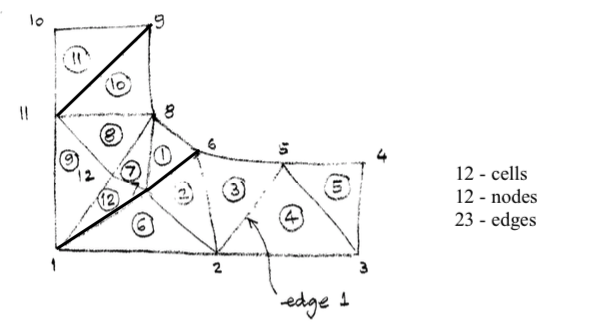
\includegraphics[width=.75\linewidth]{fig/L4_1.png}
  \caption{Sample unstructured grid.}
  \label{fig:L4_1}
\end{figure}

\section{Quasi-One-Dimensional Nozzle Flow}
\label{sec:q1dnf}


\chapter{Conclusions}
\label{ch:conc}


\clearpage
\appendix
\section*{Appendix}
\addcontentsline{toc}{section}{Appendices}
\renewcommand{\thesubsection}{\Alph{subsection}}


\subsection{Euler Equations}
\label{app:euler}
\renewcommand{\theequation}{A.\arabic{equation}}

\clearpage
%% - BIBLIOGRAPHY
\bibliographystyle{unsrt}
\bibliography{myref.bib}

\end{document}
